\documentclass[hidelinks,12pt]{article}

\renewcommand\appendix{\par
  \setcounter{section}{0}
  \setcounter{subsection}{0}
  \setcounter{figure}{0}
  \setcounter{table}{0}
  \setcounter{equation}{0}
  \renewcommand\thesection{Appendix \Alph{section}}
  \renewcommand\thefigure{\Alph{section}\arabic{figure}}
  \renewcommand\thetable{\Alph{section}\arabic{table}}
}


\newcommand{\folderTables}{"C:/Users/jbueren/Google Drive/Notes/pijoan/JMP/Model/Model_v1/tables"}

\usepackage{hyperref} 
\usepackage[margin=1.0in]{geometry}
\usepackage[utf8]{inputenc}
\usepackage[english]{babel}
 
\setlength{\parindent}{2em}
\setlength{\parskip}{0.5em}
\renewcommand{\baselinestretch}{1.0}

\usepackage{amsmath}
\usepackage{verbatim}
\usepackage{graphicx}
\usepackage{bm}
\usepackage{threeparttable}
\graphicspath{{""}}


\usepackage{epstopdf}
\usepackage{amsfonts}
\usepackage{amssymb}
\usepackage{multirow}
\usepackage{booktabs}
%\usepackage[nofiglist,notablist]{endfloat}


\usepackage[format=plain,labelfont={sc},      textfont=sc,justification=centering, labelsep=period]{caption}
\usepackage{setspace}
\usepackage{enumitem}
\def\changemargin#1#2{\list{}{\rightmargin#2\leftmargin#1}\item[]}
\let\endchangemargin=\endlist 
\usepackage{wrapfig}
\usepackage{lscape}
\usepackage{rotating}
\usepackage{lipsum}
\usepackage{bm}
\usepackage{bbm}
\usepackage{setspace}
\usepackage{cleveref}
%\usepackage[natbibapa]{apacite} 
%\bibliographystyle{apacite}

\newcommand\fnote[1]{\captionsetup{format=plain, textfont=rm,justification=raggedright}\caption*{#1}}


%\graphicspath{C:/Users/j-buer26/Google Drive/Notes/pijoan/JMP/beamer}
\def\changemargin#1#2{\list{}{\rightmargin#2\leftmargin#1}\item[]}
\let\endchangemargin=\endlist 

\title{}
\author{}


\begin{document}

\newpage
\begin{figure}
\begin{center}
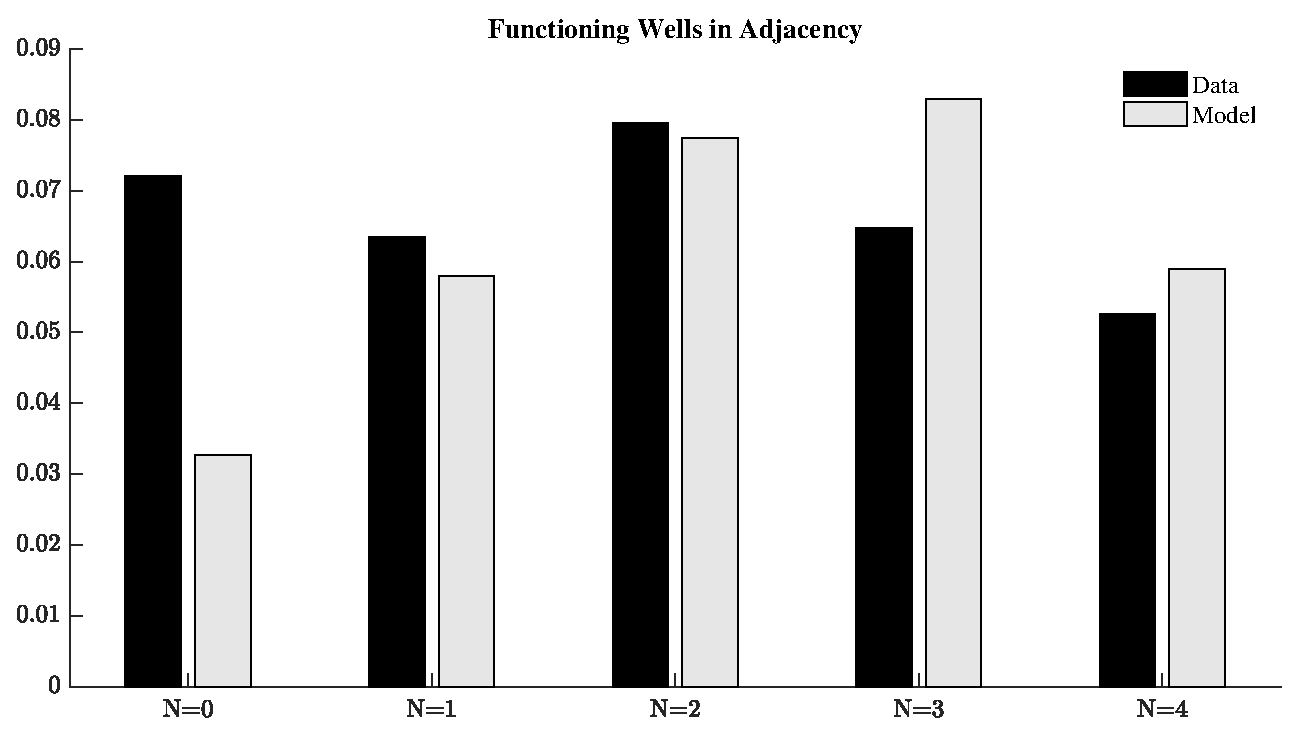
\includegraphics[scale=0.8]{model_fit2.eps}\\[20pt]
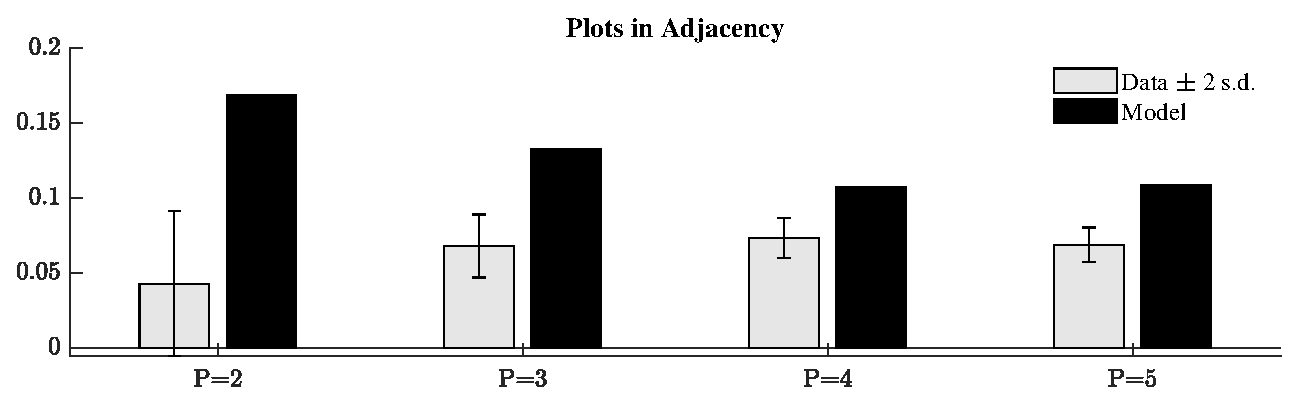
\includegraphics[scale=0.8]{model_fit4.eps}
\end{center}
\end{figure}

\begin{figure}
\begin{center}
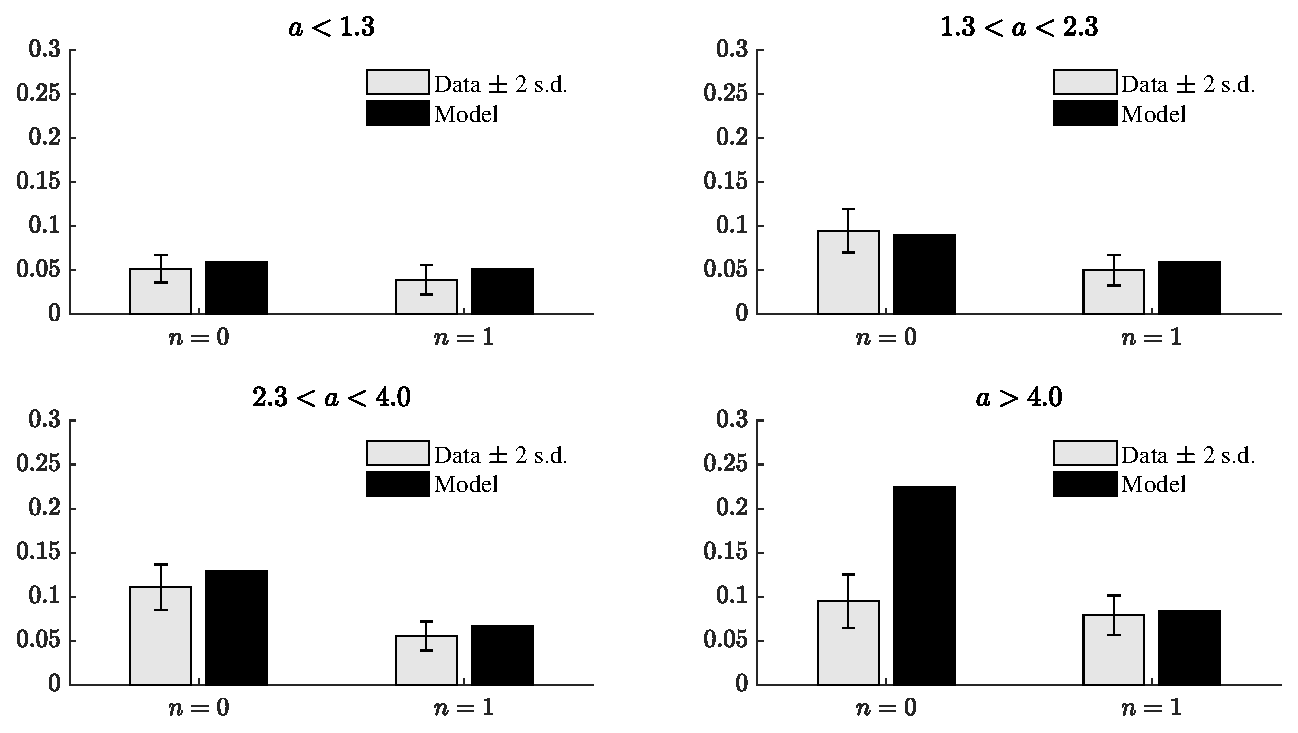
\includegraphics[scale=0.8]{model_fit3.eps}\\[20pt]
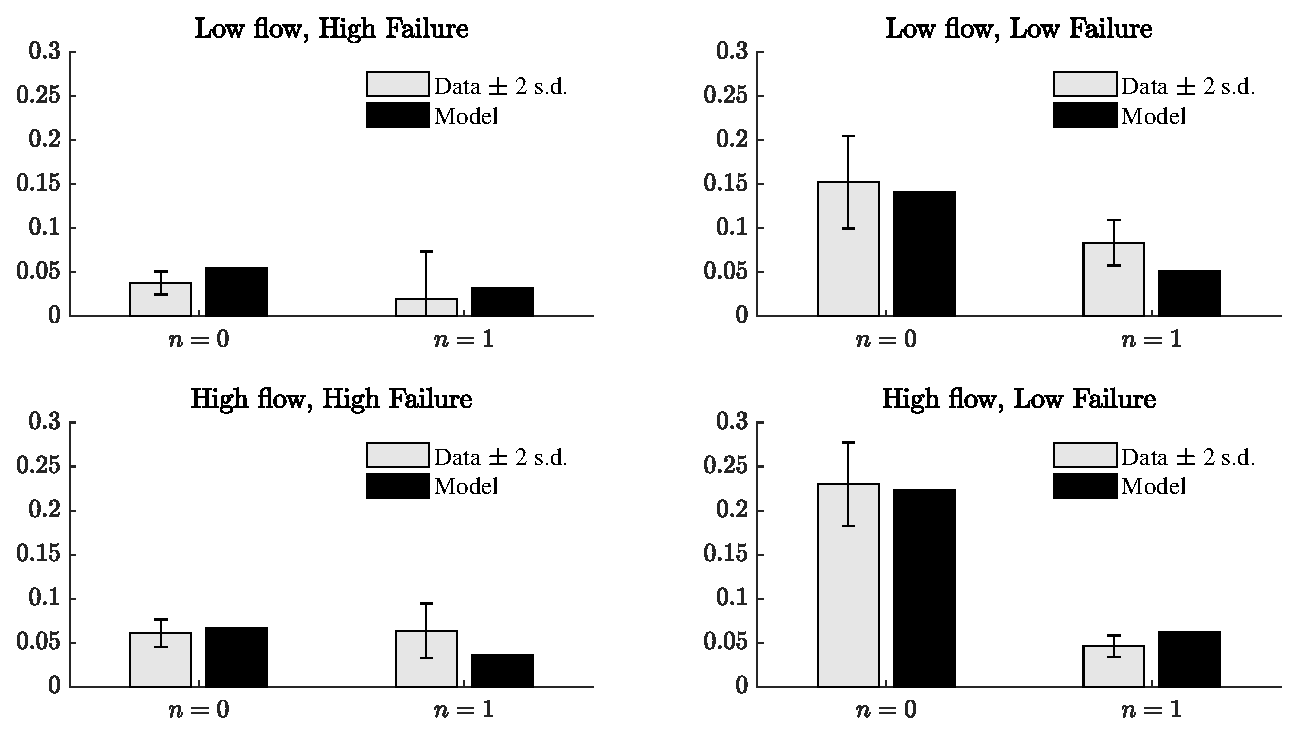
\includegraphics[scale=0.8]{model_fit5.eps}
\end{center}
\end{figure}






\end{document}

